% Created 2024-12-23 Mon 15:35
% Intended LaTeX compiler: pdflatex
\documentclass[11pt]{article}
\usepackage[utf8]{inputenc}
\usepackage[T1]{fontenc}
\usepackage{graphicx}
\usepackage{longtable}
\usepackage{wrapfig}
\usepackage{rotating}
\usepackage[normalem]{ulem}
\usepackage{amsmath}
\usepackage{amssymb}
\usepackage{capt-of}
\usepackage{hyperref}
\author{Barak-Nadav Diker}
\date{\today}
\title{Homework 1}
\hypersetup{
 pdfauthor={Barak-Nadav Diker},
 pdftitle={Homework 1},
 pdfkeywords={},
 pdfsubject={},
 pdfcreator={Emacs 29.4 (Org mode 9.7.11)}, 
 pdflang={English}}

% Setup for code blocks [1/2]

\usepackage{fvextra}

\fvset{%
  commandchars=\\\{\},
  highlightcolor=white!95!black!80!blue,
  breaklines=true,
  breaksymbol=\color{white!60!black}\tiny\ensuremath{\hookrightarrow}}

% Make line numbers smaller and grey.
\renewcommand\theFancyVerbLine{\footnotesize\color{black!40!white}\arabic{FancyVerbLine}}

\usepackage{xcolor}

% In case engrave-faces-latex-gen-preamble has not been run.
\providecolor{EfD}{HTML}{f7f7f7}
\providecolor{EFD}{HTML}{28292e}

% Define a Code environment to prettily wrap the fontified code.
\usepackage[breakable,xparse]{tcolorbox}
\DeclareTColorBox[]{Code}{o}%
{colback=EfD!98!EFD, colframe=EfD!95!EFD,
  fontupper=\footnotesize\setlength{\fboxsep}{0pt},
  colupper=EFD,
  IfNoValueTF={#1}%
  {boxsep=2pt, arc=2.5pt, outer arc=2.5pt,
    boxrule=0.5pt, left=2pt}%
  {boxsep=2.5pt, arc=0pt, outer arc=0pt,
    boxrule=0pt, leftrule=1.5pt, left=0.5pt},
  right=2pt, top=1pt, bottom=0.5pt,
  breakable}

% Support listings with captions
\usepackage{float}
\floatstyle{plain}
\newfloat{listing}{htbp}{lst}
\newcommand{\listingsname}{Listing}
\floatname{listing}{\listingsname}
\newcommand{\listoflistingsname}{List of Listings}
\providecommand{\listoflistings}{\listof{listing}{\listoflistingsname}}


% Setup for code blocks [2/2]: syntax highlighting colors

\newcommand\efstrut{\vrule height 2.1ex depth 0.8ex width 0pt}
\definecolor{EFD}{HTML}{000000}
\definecolor{EfD}{HTML}{ffffff}
\newcommand{\EFD}[1]{\textcolor{EFD}{#1}} % default
\definecolor{EFvp}{HTML}{000000}
\newcommand{\EFvp}[1]{\textcolor{EFvp}{#1}} % variable-pitch
\definecolor{EFh}{HTML}{7f7f7f}
\newcommand{\EFh}[1]{\textcolor{EFh}{#1}} % shadow
\definecolor{EFsc}{HTML}{228b22}
\newcommand{\EFsc}[1]{\textcolor{EFsc}{\textbf{#1}}} % success
\definecolor{EFw}{HTML}{ff8e00}
\newcommand{\EFw}[1]{\textcolor{EFw}{\textbf{#1}}} % warning
\definecolor{EFe}{HTML}{ff0000}
\newcommand{\EFe}[1]{\textcolor{EFe}{\textbf{#1}}} % error
\definecolor{EFl}{HTML}{ff0000}
\newcommand{\EFl}[1]{\textcolor{EFl}{#1}} % link
\definecolor{EFlv}{HTML}{ff0000}
\newcommand{\EFlv}[1]{\textcolor{EFlv}{#1}} % link-visited
\definecolor{EFhi}{HTML}{ff0000}
\newcommand{\EFhi}[1]{\textcolor{EFhi}{#1}} % highlight
\definecolor{EFc}{HTML}{b22222}
\newcommand{\EFc}[1]{\textcolor{EFc}{#1}} % font-lock-comment-face
\definecolor{EFcd}{HTML}{b22222}
\newcommand{\EFcd}[1]{\textcolor{EFcd}{#1}} % font-lock-comment-delimiter-face
\definecolor{EFs}{HTML}{8b2252}
\newcommand{\EFs}[1]{\textcolor{EFs}{#1}} % font-lock-string-face
\definecolor{EFd}{HTML}{8b2252}
\newcommand{\EFd}[1]{\textcolor{EFd}{#1}} % font-lock-doc-face
\definecolor{EFm}{HTML}{008b8b}
\newcommand{\EFm}[1]{\textcolor{EFm}{#1}} % font-lock-doc-markup-face
\definecolor{EFk}{HTML}{9370db}
\newcommand{\EFk}[1]{\textcolor{EFk}{#1}} % font-lock-keyword-face
\definecolor{EFb}{HTML}{483d8b}
\newcommand{\EFb}[1]{\textcolor{EFb}{#1}} % font-lock-builtin-face
\definecolor{EFf}{HTML}{0000ff}
\newcommand{\EFf}[1]{\textcolor{EFf}{#1}} % font-lock-function-name-face
\definecolor{EFv}{HTML}{a0522d}
\newcommand{\EFv}[1]{\textcolor{EFv}{#1}} % font-lock-variable-name-face
\definecolor{EFt}{HTML}{228b22}
\newcommand{\EFt}[1]{\textcolor{EFt}{#1}} % font-lock-type-face
\definecolor{EFo}{HTML}{008b8b}
\newcommand{\EFo}[1]{\textcolor{EFo}{#1}} % font-lock-constant-face
\definecolor{EFwr}{HTML}{ff0000}
\newcommand{\EFwr}[1]{\textcolor{EFwr}{\textbf{#1}}} % font-lock-warning-face
\newcommand{\EFnc}[1]{#1} % font-lock-negation-char-face
\definecolor{EFpp}{HTML}{483d8b}
\newcommand{\EFpp}[1]{\textcolor{EFpp}{#1}} % font-lock-preprocessor-face
\newcommand{\EFrc}[1]{\textbf{#1}} % font-lock-regexp-grouping-construct
\newcommand{\EFrb}[1]{\textbf{#1}} % font-lock-regexp-grouping-backslash
\newcommand{\EFob}[1]{#1} % org-block
\newcommand{\EFobb}[1]{#1} % org-block-begin-line
\newcommand{\EFobe}[1]{#1} % org-block-end-line
\definecolor{EFOa}{HTML}{0000ff}
\newcommand{\EFOa}[1]{\textcolor{EFOa}{#1}} % outline-1
\definecolor{EFOb}{HTML}{a0522d}
\newcommand{\EFOb}[1]{\textcolor{EFOb}{#1}} % outline-2
\definecolor{EFOc}{HTML}{a020f0}
\newcommand{\EFOc}[1]{\textcolor{EFOc}{#1}} % outline-3
\definecolor{EFOd}{HTML}{b22222}
\newcommand{\EFOd}[1]{\textcolor{EFOd}{#1}} % outline-4
\definecolor{EFOe}{HTML}{228b22}
\newcommand{\EFOe}[1]{\textcolor{EFOe}{#1}} % outline-5
\definecolor{EFOf}{HTML}{008b8b}
\newcommand{\EFOf}[1]{\textcolor{EFOf}{#1}} % outline-6
\definecolor{EFOg}{HTML}{483d8b}
\newcommand{\EFOg}[1]{\textcolor{EFOg}{#1}} % outline-7
\definecolor{EFOh}{HTML}{8b2252}
\newcommand{\EFOh}[1]{\textcolor{EFOh}{#1}} % outline-8
\definecolor{EFhn}{HTML}{008b8b}
\newcommand{\EFhn}[1]{\textcolor{EFhn}{#1}} % highlight-numbers-number
\definecolor{EFhq}{HTML}{9370db}
\newcommand{\EFhq}[1]{\textcolor{EFhq}{#1}} % highlight-quoted-quote
\definecolor{EFhs}{HTML}{008b8b}
\newcommand{\EFhs}[1]{\textcolor{EFhs}{#1}} % highlight-quoted-symbol
\definecolor{EFrda}{HTML}{707183}
\newcommand{\EFrda}[1]{\textcolor{EFrda}{#1}} % rainbow-delimiters-depth-1-face
\definecolor{EFrdb}{HTML}{7388d6}
\newcommand{\EFrdb}[1]{\textcolor{EFrdb}{#1}} % rainbow-delimiters-depth-2-face
\definecolor{EFrdc}{HTML}{909183}
\newcommand{\EFrdc}[1]{\textcolor{EFrdc}{#1}} % rainbow-delimiters-depth-3-face
\definecolor{EFrdd}{HTML}{709870}
\newcommand{\EFrdd}[1]{\textcolor{EFrdd}{#1}} % rainbow-delimiters-depth-4-face
\definecolor{EFrde}{HTML}{907373}
\newcommand{\EFrde}[1]{\textcolor{EFrde}{#1}} % rainbow-delimiters-depth-5-face
\definecolor{EFrdf}{HTML}{6276ba}
\newcommand{\EFrdf}[1]{\textcolor{EFrdf}{#1}} % rainbow-delimiters-depth-6-face
\definecolor{EFrdg}{HTML}{858580}
\newcommand{\EFrdg}[1]{\textcolor{EFrdg}{#1}} % rainbow-delimiters-depth-7-face
\definecolor{EFrdh}{HTML}{80a880}
\newcommand{\EFrdh}[1]{\textcolor{EFrdh}{#1}} % rainbow-delimiters-depth-8-face
\definecolor{EFrdi}{HTML}{887070}
\newcommand{\EFrdi}[1]{\textcolor{EFrdi}{#1}} % rainbow-delimiters-depth-9-face
\definecolor{EFany}{HTML}{CDCD00}
\newcommand{\EFany}[1]{\textcolor{EFany}{#1}} % ansi-color-yellow
\definecolor{EFanr}{HTML}{CD0000}
\newcommand{\EFanr}[1]{\textcolor{EFanr}{#1}} % ansi-color-red
\definecolor{EFanb}{HTML}{000000}
\newcommand{\EFanb}[1]{\textcolor{EFanb}{#1}} % ansi-color-black
\definecolor{EFang}{HTML}{00CD00}
\newcommand{\EFang}[1]{\textcolor{EFang}{#1}} % ansi-color-green
\definecolor{EFanB}{HTML}{0000EE}
\newcommand{\EFanB}[1]{\textcolor{EFanB}{#1}} % ansi-color-blue
\definecolor{EFanc}{HTML}{00CDCD}
\newcommand{\EFanc}[1]{\textcolor{EFanc}{#1}} % ansi-color-cyan
\definecolor{EFanw}{HTML}{E5E5E5}
\newcommand{\EFanw}[1]{\textcolor{EFanw}{#1}} % ansi-color-white
\definecolor{EFanm}{HTML}{CD00CD}
\newcommand{\EFanm}[1]{\textcolor{EFanm}{#1}} % ansi-color-magenta
\definecolor{EFANy}{HTML}{EEEE00}
\newcommand{\EFANy}[1]{\textcolor{EFANy}{#1}} % ansi-color-bright-yellow
\definecolor{EFANr}{HTML}{EE0000}
\newcommand{\EFANr}[1]{\textcolor{EFANr}{#1}} % ansi-color-bright-red
\newcommand{\EFANb}[1]{#1} % ansi-color-bright-black
\definecolor{EFANg}{HTML}{00EE00}
\newcommand{\EFANg}[1]{\textcolor{EFANg}{#1}} % ansi-color-bright-green
\definecolor{EFANB}{HTML}{0000FF}
\newcommand{\EFANB}[1]{\textcolor{EFANB}{#1}} % ansi-color-bright-blue
\definecolor{EFANc}{HTML}{00EEEE}
\newcommand{\EFANc}[1]{\textcolor{EFANc}{#1}} % ansi-color-bright-cyan
\newcommand{\EFANw}[1]{#1} % ansi-color-bright-white
\newcommand{\EFANm}[1]{#1} % ansi-color-bright-magenta
\usepackage{biblatex}

\begin{document}

\maketitle
\tableofcontents

\section{Finding the Bias Scale-Factor miss align errors}
\label{sec:org1303fa5}



Our model of errors is
\label{equ:1}
\begin{equation}
\tilde{f} = (I_3+S_a+M_a)f+b_a+w_a 
\end{equation}
Where
\begin{math}
S_a\in diag_{3\times 3}\mathbb{R}
\end{math}
and 
\begin{math}
M_a\in AntiSymm_{3\times 3}\mathbb{R}
\end{math}
and
\begin{math}
b_a\in \mathbb{R}^3
\end{math}

Note the following derivation

\begin{equation*}
\tilde{f}-f = (S_a+M_a)f+b_a
\end{equation*}
Concating the following matrices would generate the following matrix 
\begin{equation*}
M_{3\times 4}=
\left[
\begin{array}{c | c}
M_a+S_a & b_a
\end{array}
\right]
\end{equation*}

Given that \(M_{3\times 4}\) matrix we can simplify equation \ref{equ:1}
to be

\begin{equation*}
\tilde{f} - f_{3\times 1 } = M_{3\times 4}
\begin{pmatrix}
f_{3\times 1 } \\ 1 
\end{pmatrix}
\end{equation*}

For example, Estimating left column of M with down x direction measurements
\begin{equation*}
\tilde{f}_{down}^x-
\begin{pmatrix}
-g \\ 0 \\ 0 
\end{pmatrix} = M
\begin{pmatrix}
-g \\ 0 \\ 0 \\ 1
\end{pmatrix}
\end{equation*}


We can concate all the vector equations together and we'll infer the following matrix equation

\begin{equation*}
\begin{pmatrix}
\tilde{f}_{down}^{x} & \tilde{f}_{x}^{up} & \cdots & \tilde{f}_{up}^{z} 
\end{pmatrix}
-
\begin{pmatrix}
-g & g  & 0 & 0 & 0 &   0 \\
0 & 0 & -g & g & 0  & 0 \\
0 & 0 & 0 & 0  & -g & g
\end{pmatrix}
=M
\begin{pmatrix}
-g & g  &  0 & 0 & 0 & 0 \\ 
0 & 0  &  -g & g & 0  & 0 \\ 
0 & 0  &  0 & 0 & -g  & g \\ 
1 & 1 &  1 & 1 & 1 &1 \\ 
\end{pmatrix}
\end{equation*}

I'll denote the matrix \(A \in \mathbb{R}^{4\times 6 }\) like so 

\begin{equation*}
A_{4\times 6}=\begin{pmatrix}
-g & g  &  0 & 0 & 0 & 0 \\ 
0 & 0  &  -g & g & 0  & 0 \\ 
0 & 0  &  0 & 0 & -g  & g \\ 
1 & 1 &  1 & 1 & 1 &1 \\ 
\end{pmatrix}
\end{equation*}


and

\begin{equation*}
z_{3\times 6}=M_{3\times 4 }A_{4\times 6}
\end{equation*}

\begin{equation*}
z_{3\times 6}A^{T}(AA^{T})^{-1}=M_{3\times 4 }A_{4\times 6}A^{T}(AA^{T})^{-1}
\end{equation*}


\begin{equation}\label{eq:LS}
z_{3\times 6}A^{T}(AA^{T})^{-1}=M_{3\times 4 }
\end{equation}

Equation \ref{eq:LS} gives us the best \(M\) matrix for a given measurement
so our estimator is an \bold{Unbiased estimator}, so for simple calculation we'll have


\begin{equation}\label{eq:LS2}
\hat{M}=\frac{1}{n}\sum_{i=1}^{n}M = \frac{1}{n}\sum_{i=1}^{n}z_{3\times 6}A^{T}(AA^{T})^{-1}
\end{equation}
\section{Implementation}
\label{sec:orgbb5d0c7}
Here I am calculating the Matrix A of equation \ref{eq:LS} using the Following code 
\begin{Code}
\begin{Verbatim}
\color{EFD}\EFcd{\#} \EFc{Calculating A} 
\EFk{import} numpy \EFk{as} np
\EFcd{\#}\EFc{g = 9.81 \#m/s\char94{}2}
\EFv{g} =\EFhn{1} 
\EFv{D} = np.zeros((\EFhn{3},\EFhn{6}))
\EFv{D}[\EFhn{0},\EFhn{0}] = -g ; \EFv{D}[\EFhn{0},\EFhn{1}] = g ; \EFv{D}[\EFhn{1},\EFhn{2}] = -g ; \EFv{D}[\EFhn{1},\EFhn{3}] = g ; \EFv{D}[\EFhn{2},\EFhn{4}] =-g ; \EFv{D}[\EFhn{2},\EFhn{5}]=g
\EFv{E} = np.ones((\EFhn{1},\EFhn{6}),dtype=\EFb{float})
\EFb{print}(\EFs{"A="})
\EFb{print}(np.vstack((D,E)))
\end{Verbatim}
\end{Code}

\phantomsection
\label{}
\begin{verbatim}
A=
[[-1.  1.  0.  0.  0.  0.]
 [ 0.  0. -1.  1.  0.  0.]
 [ 0.  0.  0.  0. -1.  1.]
 [ 1.  1.  1.  1.  1.  1.]]
\end{verbatim}


\begin{table}[htbp]
\label{A}
\centering
\begin{tabular}{rrrrrr}
-9.81 & 9.81 & 0. & 0. & 0. & 0.\\
0. & 0. & -9.81 & 9.81 & 0. & 0.\\
0. & 0. & 0. & 0. & -9.81 & 9.81\\
1. & 1. & 1. & 1. & 1. & 1.\\
\end{tabular}
\end{table}

\begin{table}[htbp]
\label{B}
\centering
\begin{tabular}{rrrrrr}
-1. & 1. & 0. & 0. & 0. & 0.\\
0. & 0. & -1. & 1. & 0. & 0.\\
0. & 0. & 0. & 0. & -1. & 1.\\
1. & 1. & 1. & 1. & 1. & 1\\
\end{tabular}
\end{table}
\subsection{Core implementation}
\label{sec:org983c710}
Here I am finding the errors as I have developed in the theory section

In the end I'll obtain the matrix \(M\in \mathbb{R}^{3\times 4}\) which consist of \(b_a,S_a,M_a\)

\begin{Code}
\begin{Verbatim}
\color{EFD}\EFk{import} numpy \EFk{as} np
\EFk{import} pandas \EFk{as} pd
\EFv{x\_mi} = pd.read\_csv(\EFs{"./dataset\_work/sec300xminus.csv"})
\EFv{y\_mi} = pd.read\_csv(\EFs{"./dataset\_work/sec300yminus.csv"})
\EFv{z\_mi} = pd.read\_csv(\EFs{"./dataset\_work/sec300zminus.csv"})
\EFv{x\_pl} = pd.read\_csv(\EFs{"./dataset\_work/sec300xplus.csv"})
\EFv{y\_pl} = pd.read\_csv(\EFs{"./dataset\_work/sec300yplus.csv"})
\EFv{z\_pl} = pd.read\_csv(\EFs{"./dataset\_work/sec300zplus.csv"})
\EFv{x\_mi} = x\_mi[[\EFs{'gFx'},\EFs{'gFy'},\EFs{'gFz'}]].to\_numpy()
\EFv{y\_mi} = y\_mi[[\EFs{'gFx'},\EFs{'gFy'},\EFs{'gFz'}]].to\_numpy()
\EFv{z\_mi} = z\_mi[[\EFs{'gFx'},\EFs{'gFy'},\EFs{'gFz'}]].to\_numpy()
\EFv{x\_pl} = x\_pl[[\EFs{'gFx'},\EFs{'gFy'},\EFs{'gFz'}]].to\_numpy()
\EFv{y\_pl} = y\_pl[[\EFs{'gFx'},\EFs{'gFy'},\EFs{'gFz'}]].to\_numpy()
\EFv{z\_pl} = z\_pl[[\EFs{'gFx'},\EFs{'gFy'},\EFs{'gFz'}]].to\_numpy()
\EFv{A} = np.array(A)

\EFv{x\_mi} -= np.array([-\EFhn{1},\EFhn{0},\EFhn{0}])
\EFv{y\_mi} -= np.array([\EFhn{0},-\EFhn{1},\EFhn{0}])
\EFv{z\_mi} -= np.array([\EFhn{0},\EFhn{0},-\EFhn{1}])
\EFv{x\_pl} -= np.array([\EFhn{1},\EFhn{0},\EFhn{0}])
\EFv{y\_pl} -= np.array([\EFhn{0},\EFhn{1},\EFhn{0}])
\EFv{z\_pl} -= np.array([\EFhn{0},\EFhn{0},\EFhn{1}])

    
\EFv{n}=\EFhn{0} 
\EFv{sum\_of\_M} = np.zeros((\EFhn{3},\EFhn{4}))
\EFk{for} x\_m,y\_m,z\_m,x\_p,y\_p,z\_p \EFk{in} \EFb{zip}(x\_mi,y\_mi,z\_mi,x\_pl,y\_pl,z\_pl):
    \EFv{n}+=\EFhn{1}
    \EFv{x\_m} = np.expand\_dims(x\_m,\EFhn{1}).T
    \EFv{y\_m} = np.expand\_dims(y\_m,\EFhn{1}).T
    \EFv{z\_m} = np.expand\_dims(z\_m,\EFhn{1}).T
    \EFv{x\_p} = np.expand\_dims(x\_p,\EFhn{1}).T
    \EFv{y\_p} = np.expand\_dims(y\_p,\EFhn{1}).T
    \EFv{z\_p} = np.expand\_dims(z\_p,\EFhn{1}).T
    \EFv{z}= np.concatenate((x\_m,x\_p,y\_m,y\_p,z\_m,z\_p)).T
    \EFv{M}  = z @ np.transpose(A) @ np.linalg.inv(A@np.transpose(A))
    \EFv{sum\_of\_M} += M
    \EFcd{\#}\EFc{break}
\EFv{esti\_M} = sum\_of\_M/n \EFcd{\#}\EFc{, sum\_of\_M.shape}
\EFb{print}(\EFs{"The Estimated M which is unbiased estimator is} \EFo{\char92{}n}\EFs{"},esti\_M)
\EFb{print}(\EFs{"The S\_a error is} \EFo{\char92{}n}\EFs{"}, np.diag((esti\_M[\EFhn{0},\EFhn{0}],esti\_M[\EFhn{1},\EFhn{1}],esti\_M[\EFhn{2},\EFhn{2}])))
\EFv{M\_a} = esti\_M.copy()
\EFv{M\_a} = M\_a[\EFhn{0}:\EFhn{3},\EFhn{0}:\EFhn{3}]
\EFv{M\_a}[\EFhn{0},\EFhn{0}] = \EFhn{0}
\EFv{M\_a}[\EFhn{1},\EFhn{1}] = \EFhn{0}
\EFv{M\_a}[\EFhn{2},\EFhn{2}] = \EFhn{0}
\EFb{print}(\EFs{"The M\_a error is} \EFo{\char92{}n}\EFs{"}, M\_a)
\EFb{print}(\EFs{"The Bias of IMU is} \EFo{\char92{}n}\EFs{"}, esti\_M[:,\EFhn{3}])

\EFcd{\#}\EFc{return sum\_of\_M.shape}
\EFcd{\#}\EFc{return sum\_of\_M/n \#, sum\_of\_M.shape}
\EFcd{\#}\EFc{return  x\_minus[['gFx','gFy','gFz']].to\_numpy().shape[0]}
\EFcd{\#}\EFc{return x\_minus[['gFx','gFy','gFz']].to\_numpy().shape}
\end{Verbatim}
\end{Code}

\phantomsection
\label{}
\begin{verbatim}
The Estimated M which is unbiased estimator is 
 [[-0.02861075 -0.00391678 -0.01046105 -0.00122523]
 [ 0.00165313 -0.00751652 -0.00525399  0.0009181 ]
 [ 0.02379594 -0.02749688 -0.00575567  0.13867218]]
The S_a error is 
 [[-0.02861075  0.          0.        ]
 [ 0.         -0.00751652  0.        ]
 [ 0.          0.         -0.00575567]]
The M_a error is 
 [[ 0.         -0.00391678 -0.01046105]
 [ 0.00165313  0.         -0.00525399]
 [ 0.02379594 -0.02749688  0.        ]]
The Bias of IMU is 
 [-0.00122523  0.0009181   0.13867218]
\end{verbatim}
\section{2.6 Only bias error}
\label{sec:org6139c86}
In this exercise, I take only one accelerometer and consider only the bias error

for this derivation I'll consider the following equation \ref{equ:1}

\begin{equation*}
\tilde{f} = (I_3+S_a+M_a)f+b_a+w_a 
\end{equation*}

And if I am assuming only bias error, I'll have the following equation


\begin{equation}\label{equ:bias}
\tilde{f} = f+b_a 
\end{equation}
and for estimating equation \ref{equ:bias} , consider

\begin{equation}
b_a = \tilde{f}-f 
\end{equation}

which is an ``unbiased estimator''

\begin{equation}
\hat{b}_a = \frac{1}{n} \sum_{i=0}^{n} b_a = \frac{1}{n} \sum_{i=0}^{n}(\tilde{f}-f )
\end{equation}




\begin{Code}
\begin{Verbatim}
\color{EFD}\EFk{import} numpy \EFk{as} np
\EFk{import} pandas \EFk{as} pd
\EFv{x\_mi} = pd.read\_csv(\EFs{"./dataset\_work/sec300xminus.csv"})
\EFv{x\_mi} = x\_mi[[\EFs{'gFx'},\EFs{'gFy'},\EFs{'gFz'}]].to\_numpy()
\EFv{diff\_x} = x\_mi-np.array([-\EFhn{1} , \EFhn{0}, \EFhn{0}])
\EFb{print}(\EFs{"The bias of the accelerometer using average is} \EFo{\char92{}n}\EFs{"})
\EFb{print}(diff\_x.\EFb{sum}(axis=\EFhn{0}) / diff\_x.shape[\EFhn{0}])
\EFb{print}(diff\_x.shape[\EFhn{0}])
\end{Verbatim}
\end{Code}

\phantomsection
\label{}
\begin{verbatim}
The bias of the accelerometer using average is 

[ 0.02406121 -0.00294848  0.23269958]
149878
\end{verbatim}

\newpage
\section{2.7 calculate the bias errors using only average}
\label{sec:orga82b864}
In order to do so I'll Implement 2.6 for all accelerometer 

\begin{Code}
\begin{Verbatim}
\color{EFD}\EFk{import} numpy \EFk{as} np
\EFk{import} pandas \EFk{as} pd
\EFk{def} \EFf{estimate\_only\_bias}(address= \EFs{"./dataset\_work/sec300xminus.csv"},true\_force = [-\EFhn{1},\EFhn{0},\EFhn{0}]): \EFcd{\#} \EFc{true\_force = [-1,0,0]}
    \EFv{x\_mi} = pd.read\_csv(address)
    \EFv{x\_mi} = x\_mi[[\EFs{'gFx'},\EFs{'gFy'},\EFs{'gFz'}]].to\_numpy()
    \EFv{diff\_x} = x\_mi-np.array(true\_force)
    \EFk{return} diff\_x.\EFb{sum}(axis=\EFhn{0}) / diff\_x.shape[\EFhn{0}]

\EFv{bias\_term} = estimate\_only\_bias(\EFs{"./dataset\_work/sec300xminus.csv"},[-\EFhn{1},\EFhn{0},\EFhn{0}])
\EFv{bias\_term} += estimate\_only\_bias(\EFs{"./dataset\_work/sec300yminus.csv"},[\EFhn{0},-\EFhn{1},\EFhn{0}])
\EFv{bias\_term} += estimate\_only\_bias(\EFs{"./dataset\_work/sec300zminus.csv"},[\EFhn{0},\EFhn{0},-\EFhn{1}])
\EFv{bias\_term} += estimate\_only\_bias(\EFs{"./dataset\_work/sec300xplus.csv"},[\EFhn{1},\EFhn{0},\EFhn{0}])
\EFv{bias\_term} += estimate\_only\_bias(\EFs{"./dataset\_work/sec300yplus.csv"},[\EFhn{0},\EFhn{1},\EFhn{0}])
\EFv{bias\_term} += estimate\_only\_bias(\EFs{"./dataset\_work/sec300zplus.csv"},[\EFhn{0},\EFhn{0},\EFhn{1}])
\EFb{print}(\EFs{"The bias error using only averages is "})
\EFb{print}(bias\_term/\EFhn{6})
\end{Verbatim}
\end{Code}

\phantomsection
\label{}
\begin{verbatim}
The bias error using only averages is 
[-0.00119208  0.00093832  0.13886594]
\end{verbatim}
\subsection{Special note}
\label{sec:org0d8f478}
using the Entire error model the bias is very close to the average bias 

\begin{itemize}
\item The Bias of IMU using entire model  is 
{[}-0.00122523  0.0009181   0.13867218]
\item The Bias of IMU using only average is
{[}-0.00119208  0.00093832  0.13886594]
\end{itemize}
\subsection{Important conclusions}
\label{sec:orge1ed01e}
Given our entire error model lets see how well the error model fits the data by plotting the error which will be defined by \(|f - \tilde{f}|_2\) lets see how It'll look like 


our calculated \(M_{3\times 4}\) matrix is 
\begin{table}[htbp]
\label{M}
\centering
\begin{tabular}{rrrr}
-0.02861075 & -0.00391678 & -0.01046105 & -0.00122523\\
0.00165313 & -0.00751652 & -0.00525399 & 0.0009181\\
0.02379594 & -0.02749688 & -0.00575567 & 0.13867218\\
\end{tabular}
\end{table}


\begin{Code}
\begin{Verbatim}
\color{EFD}\EFk{import} numpy \EFk{as} np
\EFk{import} sys
\EFk{import} pandas \EFk{as} pd
\EFk{from} matplotlib \EFk{import} pyplot \EFk{as} plt 
\EFv{x\_mi} = pd.read\_csv(\EFs{"./dataset\_work/sec300xminus.csv"})
\EFv{y\_mi} = pd.read\_csv(\EFs{"./dataset\_work/sec300yminus.csv"})
\EFv{z\_mi} = pd.read\_csv(\EFs{"./dataset\_work/sec300zminus.csv"})
\EFv{x\_pl} = pd.read\_csv(\EFs{"./dataset\_work/sec300xplus.csv"})
\EFv{y\_pl} = pd.read\_csv(\EFs{"./dataset\_work/sec300yplus.csv"})
\EFv{z\_pl} = pd.read\_csv(\EFs{"./dataset\_work/sec300zplus.csv"})
\EFv{x\_mi} = x\_mi[[\EFs{'gFx'},\EFs{'gFy'},\EFs{'gFz'}]].to\_numpy()
\EFv{y\_mi} = y\_mi[[\EFs{'gFx'},\EFs{'gFy'},\EFs{'gFz'}]].to\_numpy()
\EFv{z\_mi} = z\_mi[[\EFs{'gFx'},\EFs{'gFy'},\EFs{'gFz'}]].to\_numpy()
\EFv{x\_pl} = x\_pl[[\EFs{'gFx'},\EFs{'gFy'},\EFs{'gFz'}]].to\_numpy()
\EFv{y\_pl} = y\_pl[[\EFs{'gFx'},\EFs{'gFy'},\EFs{'gFz'}]].to\_numpy()
\EFv{z\_pl} = z\_pl[[\EFs{'gFx'},\EFs{'gFy'},\EFs{'gFz'}]].to\_numpy()
\EFcd{\#}\EFc{A = np.array(A)}
\EFv{M} = np.array(M)
\EFv{M} = M + np.concatenate([ np.identity(\EFhn{3}) , np.array([[\EFhn{0},\EFhn{0},\EFhn{0}]]).T],axis=\EFhn{1})
\EFv{x\_mi\_improved} =x\_mi -  M @ np.array([-\EFhn{1},\EFhn{0},\EFhn{0},\EFhn{1}])
\EFv{x\_mi\_usual} =x\_mi -  np.array([-\EFhn{1},\EFhn{0},\EFhn{0}])
\EFv{y\_mi\_improved} =y\_mi -   M@np.array([\EFhn{0},-\EFhn{1},\EFhn{0},\EFhn{1}])
\EFv{y\_mi\_usual} =y\_mi -  np.array([\EFhn{0},-\EFhn{1},\EFhn{0}])
\EFv{z\_mi} -=M@np.array([\EFhn{0},\EFhn{0},-\EFhn{1},\EFhn{1}])
\EFcd{\#}\EFc{x\_pl -=M@np.array([1,0,0,1])}
\EFv{x\_pl\_improved} = x\_pl - M @np.array([\EFhn{1},\EFhn{0},\EFhn{0},\EFhn{1}])
\EFv{x\_pl\_usual} = x\_pl - np.array([\EFhn{1},\EFhn{0},\EFhn{0}])
\EFcd{\#}\EFc{print(np.linalg.norm(x\_pl\_usual[30]))}
\EFv{y\_pl} -=M@np.array([\EFhn{0},\EFhn{1},\EFhn{0},\EFhn{1}])
\EFv{z\_pl} -=M@np.array([\EFhn{0},\EFhn{0},\EFhn{1},\EFhn{1}])

\EFv{x\_mi\_improved} = np.array([np.linalg.norm(v) \EFk{for} v \EFk{in} x\_mi\_improved]).reshape(-\EFhn{1})
\EFv{x\_mi\_usual} = np.array([np.linalg.norm(v) \EFk{for} v \EFk{in} x\_mi\_usual]).reshape(-\EFhn{1})

\EFv{y\_mi\_improved} = np.array([np.linalg.norm(v) \EFk{for} v \EFk{in} y\_mi\_improved]).reshape(-\EFhn{1})
\EFv{y\_mi\_usual} = np.array([np.linalg.norm(v) \EFk{for} v \EFk{in} y\_mi\_usual]).reshape(-\EFhn{1})
\EFv{x\_pl\_improved} = np.array([np.linalg.norm(v) \EFk{for} v \EFk{in} x\_pl\_improved]).reshape(-\EFhn{1})
\EFv{x\_pl\_usual} = np.array([np.linalg.norm(v) \EFk{for} v \EFk{in} x\_pl\_usual]).reshape(-\EFhn{1})
\EFcd{\#}\EFc{print(x\_mi[:3])}
\EFv{fig}, \EFv{ax} = plt.subplots(\EFhn{3},\EFhn{1},figsize=(\EFhn{5},\EFhn{10}))
ax[\EFhn{0}].set\_title(\EFs{"x minus before and after calibration"})
ax[\EFhn{0}].plot(np.arange(\EFb{len}(x\_mi[:\EFhn{200}])),x\_mi\_improved[:\EFhn{200}],\EFs{'+'},label=\EFs{'After Calibration'})
ax[\EFhn{0}].plot(np.arange(\EFb{len}(x\_mi[:\EFhn{200}])),x\_mi\_usual[:\EFhn{200}],label=\EFs{'Before calibration'})
ax[\EFhn{0}].legend()
ax[\EFhn{1}].set\_title(\EFs{"y minus before and after calibration"})
ax[\EFhn{1}].plot(np.arange(\EFb{len}(y\_mi[:\EFhn{200}])),y\_mi\_improved[:\EFhn{200}],\EFs{'+'},label=\EFs{'After Calibration'})
ax[\EFhn{1}].plot(np.arange(\EFb{len}(y\_mi[:\EFhn{200}])),y\_mi\_usual[:\EFhn{200}],label=\EFs{'Before calibration'})
ax[\EFhn{1}].legend()
ax[\EFhn{2}].set\_title(\EFs{"x plus before and after calibration"})
ax[\EFhn{2}].plot(np.arange(\EFb{len}(x\_pl[:\EFhn{200}])),x\_pl\_improved[:\EFhn{200}],\EFs{'+'},label=\EFs{'After Calibration'})
ax[\EFhn{2}].plot(np.arange(\EFb{len}(x\_pl[:\EFhn{200}])),x\_pl\_usual[:\EFhn{200}],label=\EFs{'Before calibration'})
ax[\EFhn{2}].legend()
plt.xlabel(\EFs{"Sample[1]"})
plt.ylabel(\EFs{"Error in eulidean norm[g]"})
plt.ylim(-\EFhn{0.001},\EFhn{0.3})
plt.savefig(\EFs{'error\_fixed\_unfixed.png'})
\EFcd{\#}\EFc{plt.show()}
    
\end{Verbatim}
\end{Code}

\begin{center}
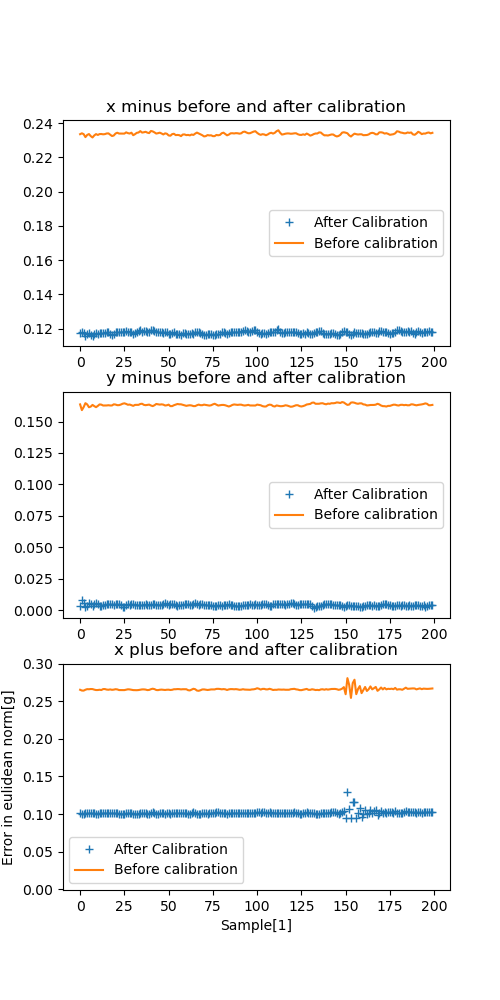
\includegraphics[width=.9\linewidth]{./error_fixed_unfixed.png}
\end{center}
\end{document}
